% Ημερίδα πρακτικής άσκησης με δεδομένα από το CERN - Σάββατο 7 Μάρτη 9:00 - 17:00
\begin{MyArticle}[enhanced, tikz={rotate=0}, width=0.6\textwidth]{Master of Masterclasses \ldots}
  \begin{multicols}{2}
    Another particle physics 
    masterclass was organized at the University of Cyprus by the
    Department of Physics. Thisyear the interest in this event was
    unique and particularlyencouraging. The day \say{Practical Experience with data analysis from
    CERN} was organized by Professor Fotios Ptochos for the 8$^{th}$ year
    in a row and took place within the framework of the
    International Particle Physics Outreach Group (IPPOG)
    effort with the aim of informing the general
    public and especially you students about the research that is
    carried out not only in CERN but also in the wider field of
    Particle Physics. The event you took place on Saturday 07 March
    2020 at the University of Cyprus Campus between 9:00 - 17:00. It 
    included lectures about the world of elementary particles,
    detection methods, and the technology developed starting with basic research in both this and
    related fields of physics. Students had a unique opportunity to
    analyze data from proton-proton collisions, as recorded by the CMS
    detector at CERN's Large Hadron Collider (LHC). They discussed their
    findings with students from other countries as well as scientists
    at CERN through a video conference, during which they also had the
    opportunity to address questions to CERN scientists. 
    % No prior knowledge of particle physics is required, but you may find
    % it easier to read some things before the workshop so you can ask more
    % questions. I am giving you some links below where you can find a lot
    % of information either in English or in Greek:
    % ========================
    \begin{figure}
      \begin{center}
        \leavevmode
        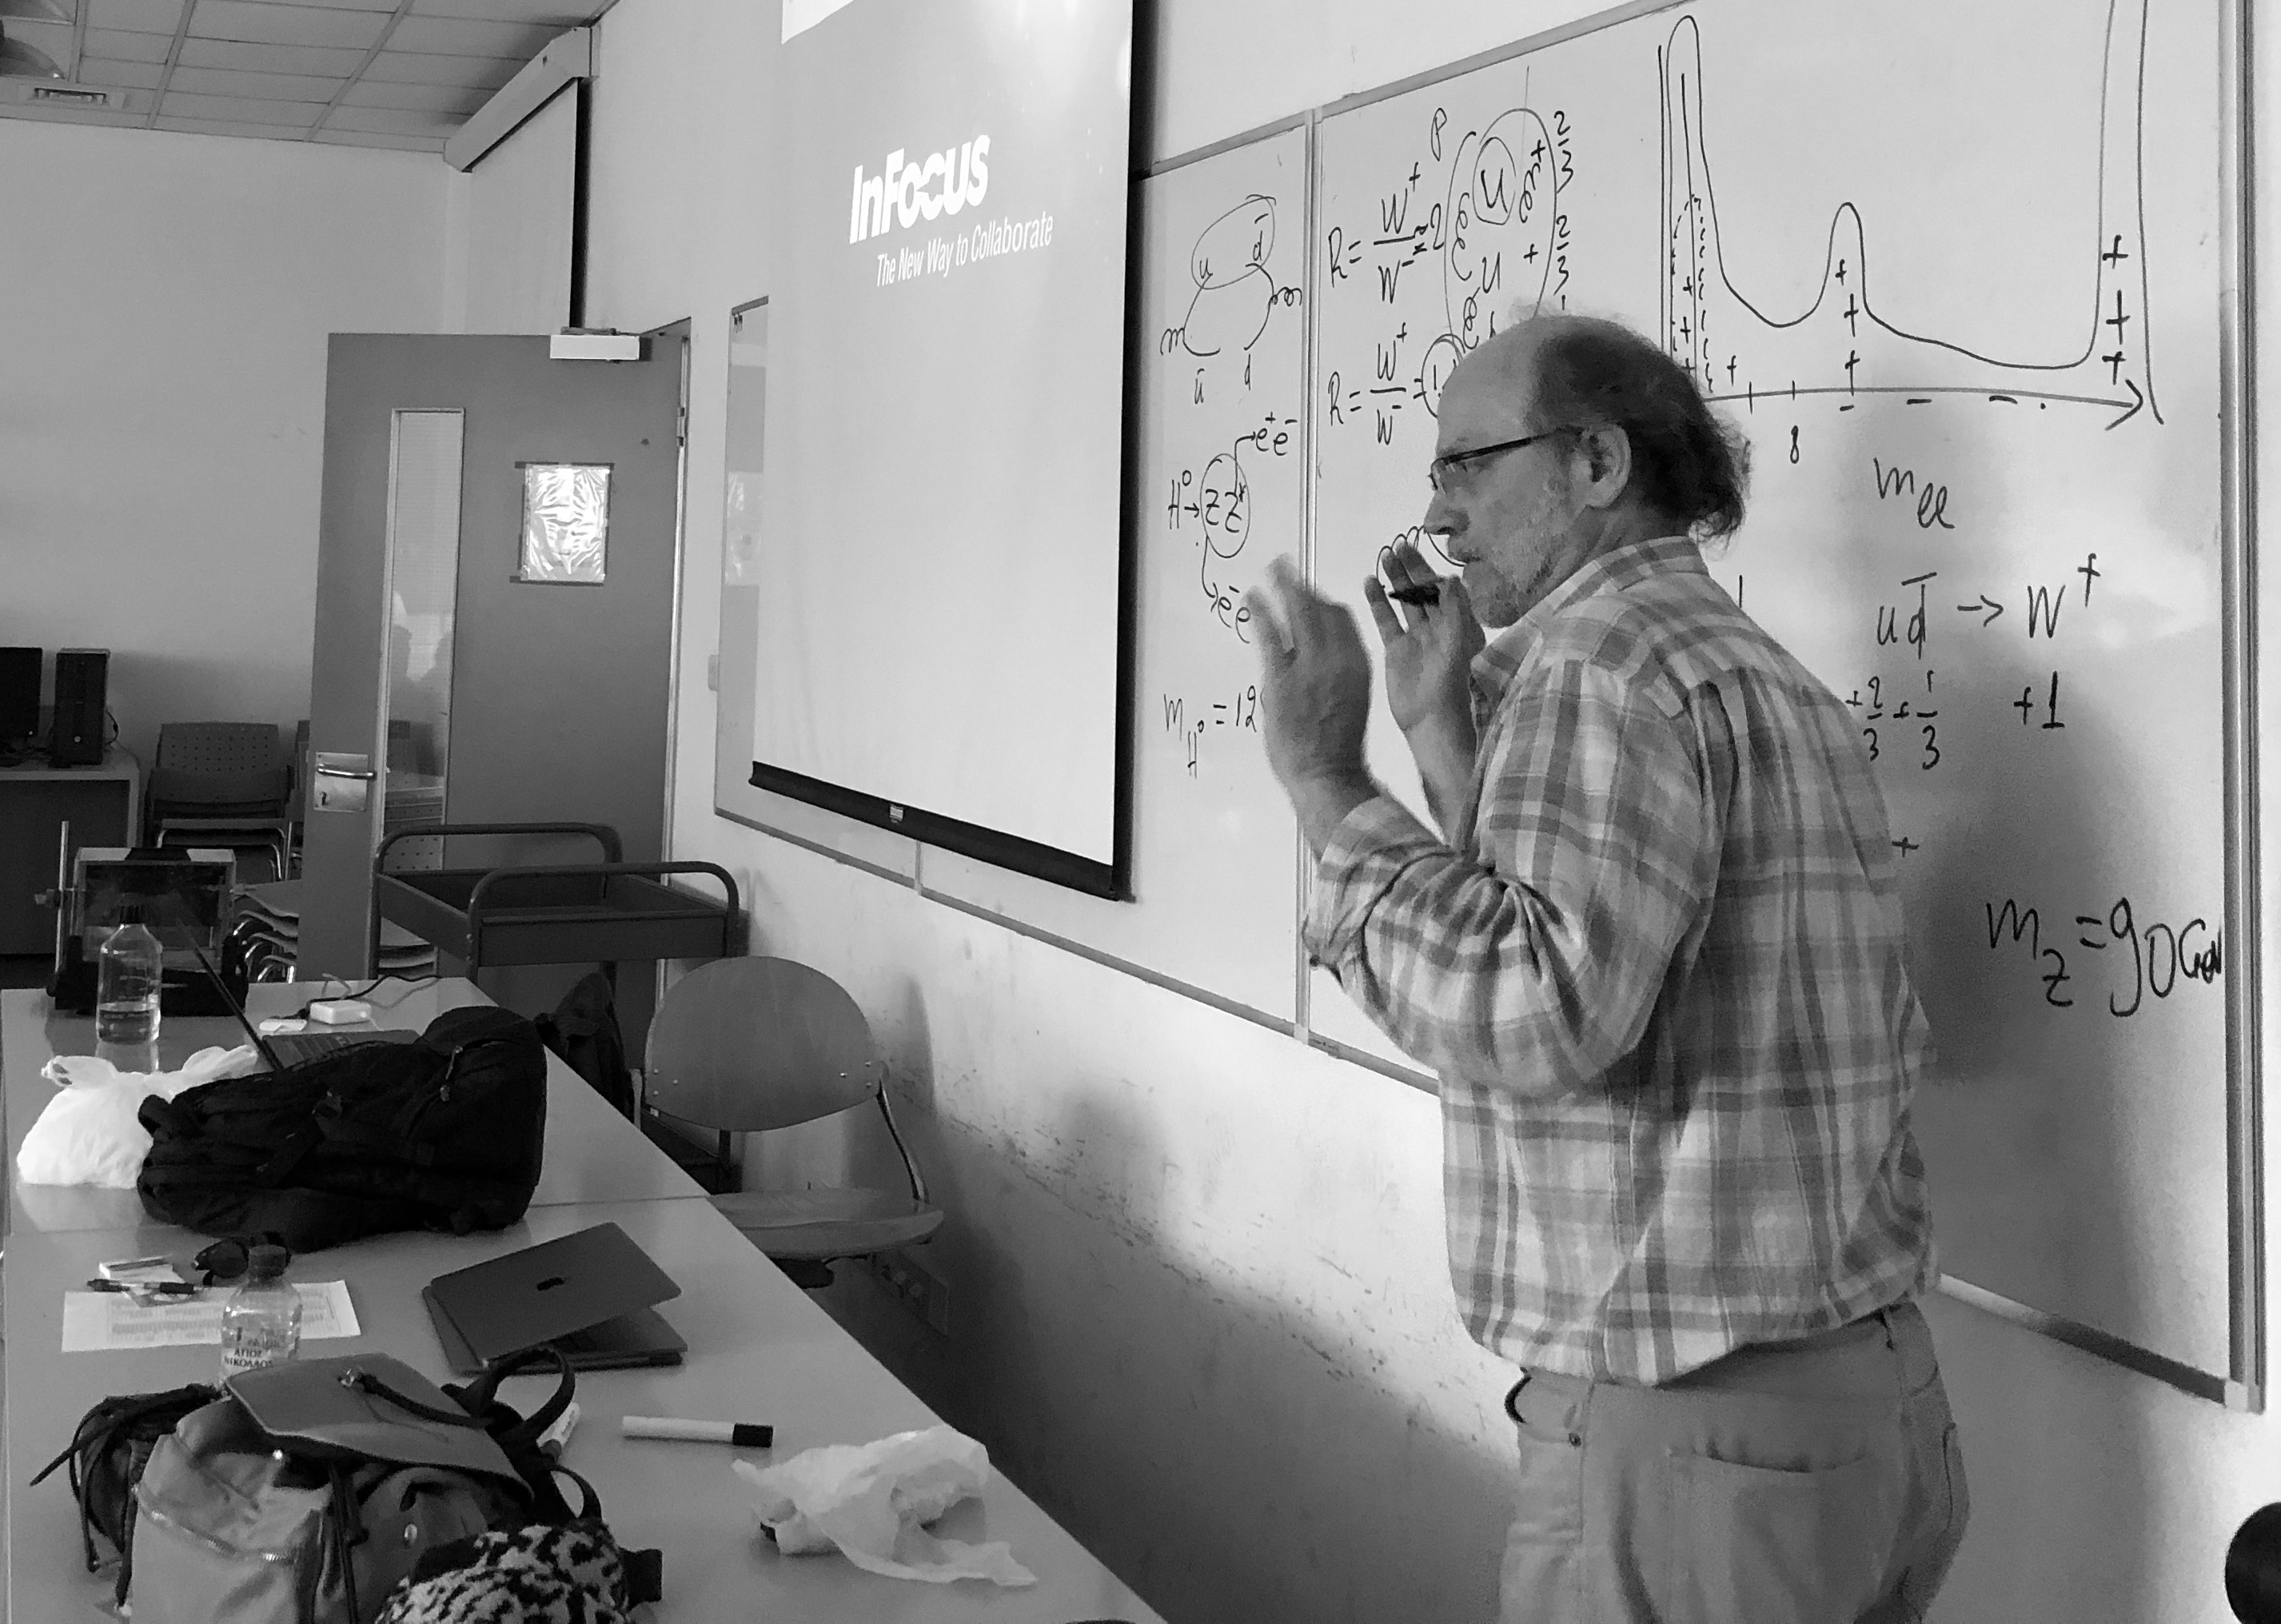
\includegraphics[width=0.45\textwidth]{./figures/Fotis6.png}
      \end{center}
    \end{figure}
    % ========================
  \end{multicols}
\end{MyArticle}
